\documentclass[12pt,a4paper]{report}

% --- Essential Packages ---
\usepackage[utf8]{inputenc}
\usepackage[margin=1in]{geometry}
\usepackage{graphicx}
\usepackage{amsmath,amssymb}
\usepackage{booktabs}
\usepackage{tabularx}
\usepackage{xcolor}
\usepackage{titlesec}
\usepackage{fancyhdr}
\usepackage{hyperref}
\usepackage{listings}
\usepackage{tikz}
\usetikzlibrary{shapes.geometric, arrows, positioning, fit, backgrounds}

% --- Color Palette ---
\definecolor{vitblue}{RGB}{0, 48, 135}
\definecolor{vitaccent}{RGB}{200, 16, 46}
\definecolor{darkgray}{RGB}{50, 50, 50}
\definecolor{codebg}{RGB}{245, 247, 250}
\definecolor{codeframe}{RGB}{200, 205, 215}

% --- Hyperlink Setup ---
\hypersetup{
    colorlinks=true,
    linkcolor=vitblue,
    citecolor=vitaccent,
    urlcolor=vitblue
}

% --- Header & Footer Configuration ---
\pagestyle{fancy}
\fancyhf{}
\fancyhead[L]{\small\color{darkgray}Student Result Management System (SRMS)}
\fancyhead[R]{\small\color{darkgray}VIT Bhopal University}
\fancyfoot[L]{\small\color{darkgray}BUDDHA S (25BAI11592)}
\fancyfoot[R]{\thepage}
\renewcommand{\headrulewidth}{0.4pt}
\renewcommand{\footrulewidth}{0.4pt}

% --- Code Listing Style ---
\lstset{
    backgroundcolor=\color{codebg},
    basicstyle=\ttfamily\footnotesize,
    keywordstyle=\color{vitblue}\bfseries,
    commentstyle=\color{gray}\itshape,
    stringstyle=\color{vitaccent},
    frame=single,
    rulecolor=\color{codeframe},
    breaklines=true,
    numbers=left,
    numberstyle=\tiny\color{gray},
    showstringspaces=false,
    tabsize=4
}

% --- Document Formatting ---
\titleformat{\chapter}[display]
  {\normalfont\bfseries\color{vitblue}}{\chaptertitlename\ \thechapter}{14pt}{\Large}
\titlespacing*{\chapter}{0pt}{-20pt}{20pt}

\begin{document}

% =========================================================================
% COVER PAGE
% =========================================================================
\begin{titlepage}
    \centering
    \vspace*{0.5cm}
    
    {\Large\textbf{\color{vitblue}VELLORE INSTITUTE OF TECHNOLOGY (VIT), BHOPAL}}\\[0.3cm]
    {\large School of Computing Science and Engineering (SCSE)}\\[0.2cm]
    {\small Bhopal-Indore Highway, Kothrikalan, Sehore, Madhya Pradesh - 466114}\\[1.2cm]

    % --- Centered VIT Bhopal Logo ---
    \begin{center}
        
\includegraphics[width=0.65\textwidth]{assets/vit_bhopal_logo.png}
    \end{center}
    
    \vspace{1.0cm}
    
    {\Huge\textbf{\color{vitblue}PROJECT REPORT}}\\[0.4cm]
    \rule{\textwidth}{1.5pt}\\[0.4cm]
    {\LARGE\textbf{STUDENT RESULT MANAGEMENT SYSTEM (SRMS)}}\\[0.3cm]
    {\large\textit{A Modular, Object-Oriented Academic Evaluation and Performance Analytics Suite}}\\[0.2cm]
    \rule{\textwidth}{1.5pt}\\[1.0cm]
    
    \textbf{\color{vitaccent}VITyarthi -- Build Your Own Project (Flipped Course Evaluation)}\\[0.2cm]
    Course: Object-Oriented Programming in Java\\[1.5cm]
    
    \begin{minipage}{0.48\textwidth}
        \flushleft
        \textbf{Submitted By:}\\[0.2cm]
        \textbf{BUDDHA S}\\
        Registration No: \textbf{25BAI11592}\\
        B.Tech in Artificial Intelligence \& ML\\
        VIT Bhopal University
    \end{minipage}
    \hfill
    \begin{minipage}{0.48\textwidth}
        \flushright
        \textbf{Evaluation Details:}\\[0.2cm]
        Academic Year: 2025--2026\\
        Flipped Class Project Component\\
        Department of Computer Science\\
        VIT Bhopal University
    \end{minipage}

    \vfill
    {\small Academic Session 2025--2026}
\end{titlepage}

% =========================================================================
% ABSTRACT / DECLARATION
% =========================================================================
\chapter*{Declaration \& Abstract}
\addcontentsline{toc}{chapter}{Declaration \& Abstract}

\section*{Student Declaration}
I hereby declare that the project entitled \textbf{``Student Result Management System (SRMS)''} submitted in partial fulfillment of the continuous flipped evaluation under the \textbf{VITyarthi -- Build Your Own Project} initiative is a record of original, independent engineering work carried out by me. All algorithms, class architectures, exception models, and data validation rules have been authored cleanly and aligned with academic integrity standards.

\vspace{1.0cm}
\noindent
\textbf{BUDDHA S}\\
Registration No: \textbf{25BAI11592}\\
School of Computing Science and Engineering (SCSE)\\
Vellore Institute of Technology (VIT), Bhopal

\vspace{1.5cm}
\hrule
\vspace{0.8cm}

\section*{Abstract}
The \textbf{Student Result Management System (SRMS)} is an industrial-standard, object-oriented console application engineered in Java to automate the end-to-end academic evaluation lifecycle within higher education departments. Traditional spreadsheet-based grade compilation workflows are prone to calculation errors, permit corrupt or negative data entries, lack duplicate-key prevention, and do not provide real-time analytical insights into student cohort performance.

The SRMS addresses these challenges through a modular three-tier architecture encompassing: (1) an encapsulated domain model with domain-specific invariants and boundary guards, (2) an automated academic calculation engine adhering to the institutional 10-point GPA and Letter Grade ($A^+$ through $F$) scale, (3) a statistical intelligence module that computes batch central tendencies, subject-wise extrema, and ASCII performance distributions, (4) a persistent CSV storage engine with fault-tolerant error recovery, and (5) a robust console interface with defensive input parsing. An automated verification test suite consisting of 12 unit test cases confirms 100\% mathematical accuracy and data integrity across all lifecycle operations.

\tableofcontents
\newpage

% =========================================================================
% CHAPTER 1: INTRODUCTION
% =========================================================================
\chapter{Introduction}

\section{Background \& Motivation}
Academic record management represents a critical operational pillar for universities, institutes, and departments. At institutions like Vellore Institute of Technology (VIT), thousands of students are evaluated across multiple technical courses each term. In smaller departments or specialized modular classes, instructors frequently resort to ad-hoc calculation tools or spreadsheet documents. While functional for basic data entry, spreadsheets lack strict type checking, fail to enforce entity integrity, allow contradictory grade entries, and require manual compilation for statistical insights.

\section{Project Objectives}
The primary objective of this project is to develop a standalone, enterprise-grade, object-oriented Java software application that models, computes, analyzes, and persists student academic records. Specifically, the project aims to:
\begin{enumerate}
    \item Implement complete CRUD (Create, Read, Update, Delete) record lifecycle management with zero tolerance for duplicate student identification numbers.
    \item Enforce mathematical and domain validity across all score entries (restricting subject marks to $[0.0, 100.0]$).
    \item Standardize academic grading through automated computation of total marks, aggregate percentages, 10-point GPA, letter grades ($A^+$ through $F$), and performance remarks.
    \item Provide real-time batch statistical analytics, including class topper recognition, lowest score tracking, pass/fail ratios, and subject-wise averages.
    \item Ensure durable data persistence through comma-separated values (CSV) file serialization and deserialization.
    \item Guarantee zero unexpected crashes through structured custom exception handling and defensive CLI input stream parsing.
\end{enumerate}

% =========================================================================
% CHAPTER 2: PROBLEM STATEMENT & SCOPE
% =========================================================================
\chapter{Problem Statement \& Scope}

\section{Problem Statement}
In conventional, non-automated academic grading environments:
\begin{itemize}
    \item \textbf{Human Computational Errors}: Manual aggregation of marks and percentage calculations frequently introduce rounding discrepancies and incorrect grade assignments.
    \item \textbf{Lack of Invariant Validation}: Systems without runtime boundary checks permit negative marks, scores above maximum ceilings, or unassigned student identifiers.
    \item \textbf{Data Duplication}: Without primary key validation, students can inadvertently be assigned multiple conflicting records.
    \item \textbf{Analytical Inefficiency}: Determining cohort pass rates, highest/lowest subject marks, and class distribution curves requires labor-intensive external recalculation.
    \item \textbf{Session Volatility}: In-memory script tools lose all accumulated records upon terminal closure, jeopardizing academic records.
\end{itemize}

\section{Scope of the System}
\begin{itemize}
    \item \textbf{Functional Scope}: Supports multi-subject evaluation in core technical subjects (\textit{Mathematics}, \textit{Java Programming}, and \textit{Physics}), individual report card generation, tabular roster generation, full-text and ID search, ranked merit leaderboard display, and CSV data synchronization.
    \item \textbf{Target Users}: Academic instructors, course coordinators, department heads, and examination cell evaluators.
    \item \textbf{Boundary}: Single-node desktop console system designed for high computational speed, local file storage, and lightweight memory footprint.
\end{itemize}

% =========================================================================
% CHAPTER 3: REQUIREMENTS SPECIFICATION
% =========================================================================
\chapter{Requirements Specification}

\section{Functional Requirements (FR)}
\begin{itemize}
    \item \textbf{FR-1: Student Enrollment (Create)}: The system shall accept a unique positive integer ID, non-empty full name, and marks for Mathematics, Java, and Physics. Registration must be blocked if the ID already exists.
    \item \textbf{FR-2: Record Inspection (Read)}: The system shall render all stored student records in an aligned, bordered ASCII grid table showing raw marks, totals, percentages, letter grades, GPAs, and pass/fail statuses.
    \item \textbf{FR-3: Dual Query Search}: The system shall enable retrieval by exact numeric ID (producing an official formatted report card) or case-insensitive name substrings.
    \item \textbf{FR-4: Score Revision (Update)}: Instructors shall be permitted to update individual subject marks with automatic re-validation and instant grade recomputation.
    \item \textbf{FR-5: Record Deletion (Delete)}: The system shall allow permanent deletion of records matching an ID, requiring explicit user confirmation.
    \item \textbf{FR-6: Academic Merit Ranking}: The system shall sort and display all students in descending order of percentage aggregate (Class Leaderboard).
    \item \textbf{FR-7: Analytical Intelligence}: The system shall compute overall pass rates, identify class toppers and lowest scorers, calculate subject-wise averages and extrema, and display an ASCII grade distribution histogram.
    \item \textbf{FR-8: Data Persistence}: The system shall export memory records to \texttt{students\_data.csv} and restore records seamlessly across application restarts.
    \item \textbf{FR-9: Demo Data Seeding}: The system shall offer a one-click sample seeder to load diverse benchmark records for quick evaluation and vivas.
\end{itemize}

\section{Non-Functional Requirements (NFR)}
\begin{itemize}
    \item \textbf{NFR-1: Robust Error Handling \& Fault Tolerance}: The system shall catch invalid user inputs, format mismatches, and domain violations gracefully using custom exceptions without terminating the runtime process.
    \item \textbf{NFR-2: Usability \& Terminal UX}: Menu options must be clearly numbered, prompts must specify acceptable bounds, and outputs must utilize visual dividers and aligned columns.
    \item \textbf{NFR-3: Maintainability \& Modularity}: Implementation must adhere to SOLID design principles, dividing responsibilities cleanly into models, service controllers, presentation utilities, and persistence managers.
    \item \textbf{NFR-4: Data Integrity}: Collections returned by service layers must be unmodifiable (\texttt{Collections.unmodifiableList}) to protect in-memory state against accidental caller mutations.
    \item \textbf{NFR-5: Computational Efficiency}: All calculation routines must execute in $O(1)$ time complexity per student, and search queries must complete within $O(n)$ time.
\end{itemize}

% =========================================================================
% CHAPTER 4: SYSTEM ARCHITECTURE & DESIGN
% =========================================================================
\chapter{System Architecture \& Design}

\section{Architectural Overview}
The system employs a decoupled, layered architectural model consisting of three distinct layers:
\begin{enumerate}
    \item \textbf{Presentation Tier}: Encapsulated by \texttt{Main.java} (interactive CLI loop) and \texttt{TableFormatter.java} (ASCII layout engine).
    \item \textbf{Service \& Business Logic Tier}: Encapsulated by \texttt{StudentManager.java} (repository/controller), \texttt{ResultCalculator.java} (grading engine), and \texttt{Statistics.java} (analytics processor).
    \item \textbf{Domain \& Persistence Tier}: Encapsulated by the \texttt{Student.java} entity and \texttt{FileStorageService.java} (CSV I/O).
\end{enumerate}

\section{System Architecture Diagram}
\begin{figure}[htbp]
\centering
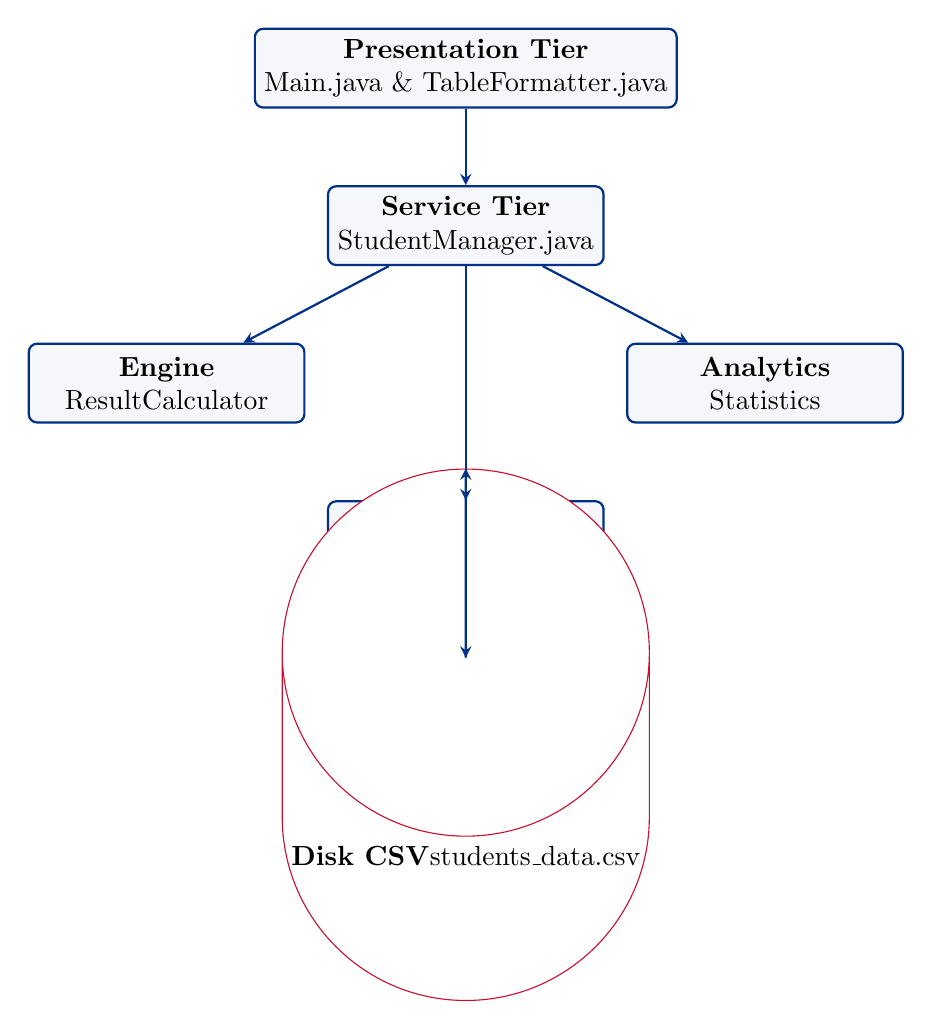
\begin{tikzpicture}[
    box/.style={rectangle, draw=vitblue, fill=codebg, thick, minimum width=3.5cm, minimum height=1.0cm, align=center, rounded corners=3pt},
    arrow/.style={thick, ->, >=stealth, color=vitblue}
]
    \node[box] (cli) at (0, 4) {\textbf{Presentation Tier}\\Main.java \& TableFormatter.java};
    \node[box] (mgr) at (0, 2) {\textbf{Service Tier}\\StudentManager.java};
    \node[box] (calc) at (-3.8, 0) {\textbf{Engine}\\ResultCalculator};
    \node[box] (stat) at (3.8, 0) {\textbf{Analytics}\\Statistics};
    \node[box] (model) at (0, -2) {\textbf{Domain Model}\\Student.java};
    \node[box] (storage) at (0, -4) {\textbf{Persistence Tier}\\FileStorageService.java};
    \node[cylinder, shape border rotate=90, draw=vitaccent, fill=white, minimum width=2.5cm, minimum height=1.0cm] (disk) at (0, -6) {\textbf{Disk CSV}\\students\_data.csv};

    \draw[arrow] (cli) -- (mgr);
    \draw[arrow] (mgr) -- (calc);
    \draw[arrow] (mgr) -- (stat);
    \draw[arrow] (mgr) -- (model);
    \draw[arrow] (mgr) -- (storage);
    \draw[arrow] (storage) -- (disk);
\end{tikzpicture}
\caption{Three-Tier Architecture of the Student Result Management System.}
\end{figure}

\section{Process Workflow Diagram}
\begin{figure}[htbp]
\centering
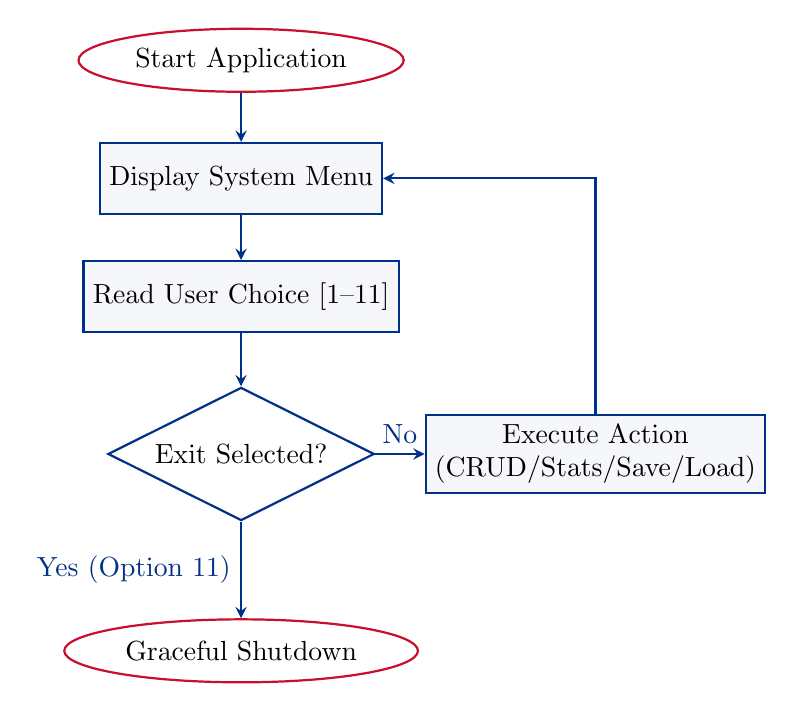
\begin{tikzpicture}[
    startstop/.style={ellipse, draw=vitaccent, fill=white, thick, minimum width=2.5cm, minimum height=0.8cm, align=center},
    process/.style={rectangle, draw=vitblue, fill=codebg, thick, minimum width=3.5cm, minimum height=0.9cm, align=center},
    decision/.style={diamond, aspect=2, draw=vitblue, fill=white, thick, align=center},
    arrow/.style={thick, ->, >=stealth, color=vitblue}
]
    \node[startstop] (start) at (0, 6) {Start Application};
    \node[process] (menu) at (0, 4.5) {Display System Menu};
    \node[process] (input) at (0, 3) {Read User Choice [1--11]};
    \node[decision] (dec) at (0, 1) {Exit Selected?};
    \node[process] (action) at (4.5, 1) {Execute Action\\(CRUD/Stats/Save/Load)};
    \node[startstop] (stop) at (0, -1.5) {Graceful Shutdown};

    \draw[arrow] (start) -- (menu);
    \draw[arrow] (menu) -- (input);
    \draw[arrow] (input) -- (dec);
    \draw[arrow] (dec) -- node[left] {Yes (Option 11)} (stop);
    \draw[arrow] (dec) -- node[above] {No} (action);
    \draw[arrow] (action) |- (menu);
\end{tikzpicture}
\caption{Interactive System Execution Workflow.}
\end{figure}

\section{Sequence Diagram: Student Enrollment}
\begin{figure}[htbp]
\centering
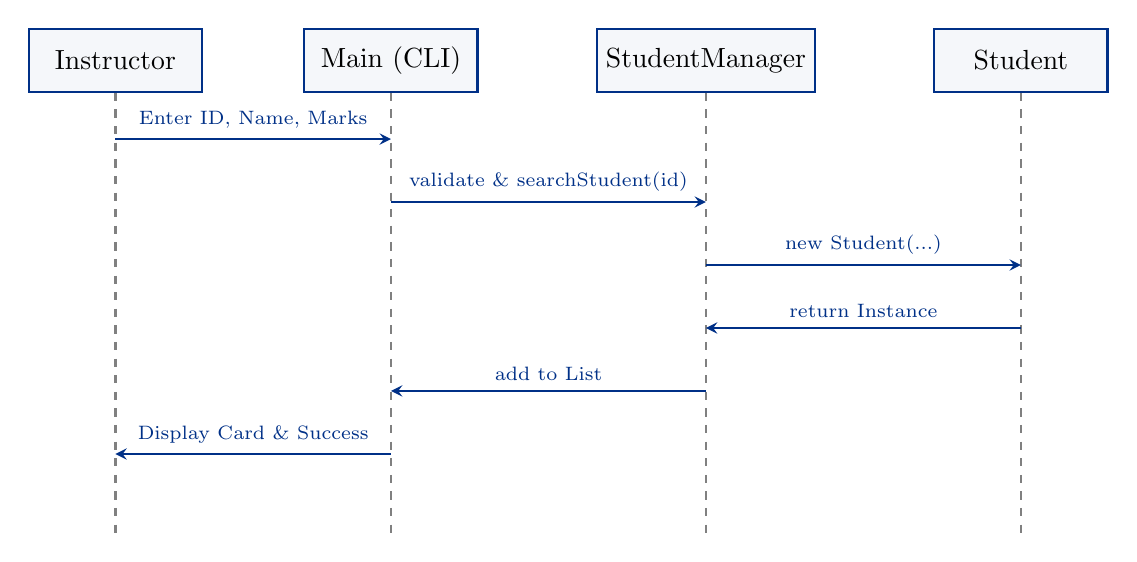
\begin{tikzpicture}[
    lifeline/.style={thick, dashed, color=gray},
    entity/.style={rectangle, draw=vitblue, fill=codebg, thick, minimum width=2.2cm, minimum height=0.8cm, align=center},
    msg/.style={thick, ->, >=stealth, color=vitblue}
]
    \node[entity] (user) at (0, 6) {Instructor};
    \node[entity] (main) at (3.5, 6) {Main (CLI)};
    \node[entity] (mgr) at (7.5, 6) {StudentManager};
    \node[entity] (st) at (11.5, 6) {Student};

    \draw[lifeline] (user) -- (0, 0);
    \draw[lifeline] (main) -- (3.5, 0);
    \draw[lifeline] (mgr) -- (7.5, 0);
    \draw[lifeline] (st) -- (11.5, 0);

    \draw[msg] (0, 5) -- node[above]{\scriptsize Enter ID, Name, Marks} (3.5, 5);
    \draw[msg] (3.5, 4.2) -- node[above]{\scriptsize validate \& searchStudent(id)} (7.5, 4.2);
    \draw[msg] (7.5, 3.4) -- node[above]{\scriptsize new Student(...)} (11.5, 3.4);
    \draw[msg] (11.5, 2.6) -- node[above]{\scriptsize return Instance} (7.5, 2.6);
    \draw[msg] (7.5, 1.8) -- node[above]{\scriptsize add to List} (3.5, 1.8);
    \draw[msg] (3.5, 1.0) -- node[above]{\scriptsize Display Card \& Success} (0, 1.0);
\end{tikzpicture}
\caption{UML Sequence Diagram for Student Record Enrollment.}
\end{figure}

\section{Class Diagram}
\begin{figure}[htbp]
\centering
\begin{tikzpicture}[
    classbox/.style={rectangle, draw=vitblue, fill=codebg, thick, minimum width=6cm, align=left, font=\scriptsize\ttfamily}
]
    \node[classbox] (st) at (0, 4) {
        \textbf{\large Student}\\
        \hline
        - id: int\\
        - name: String\\
        - maths: double\\
        - java: double\\
        - physics: double\\
        \hline
        + getId(): int\\
        + getName(): String\\
        + getMaths(): double\\
        + setMaths(m: double): void\\
        + updateMarks(m, j, p): void\\
        + toString(): String
    };

    \node[classbox] (calc) at (8, 4) {
        \textbf{\large ResultCalculator}\\
        \hline
        + PASSING\_MARK: double = 40.0\\
        + TOTAL\_SUBJECTS: int = 3\\
        \hline
        + getTotal(s: Student): double\\
        + getPercentage(s: Student): double\\
        + isPassed(s: Student): boolean\\
        + getGrade(s: Student): String\\
        + getGPA(s: Student): double\\
        + getRemark(s: Student): String
    };

    \node[classbox] (mgr) at (4, -1) {
        \textbf{\large StudentManager}\\
        \hline
        - students: List$<$Student$>$\\
        - storageService: FileStorageService\\
        \hline
        + addStudent(s: Student): boolean\\
        + searchStudent(id: int): Student\\
        + searchByName(query: String): List\\
        + updateStudentMarks(id, m, j, p): void\\
        + deleteStudent(id: int): boolean\\
        + getStudentsSortedByRank(): List\\
        + seedSampleData(): void
    };

    \draw[thick, ->, >=stealth, color=vitblue] (mgr) -- (st);
    \draw[thick, ->, >=stealth, color=vitblue] (mgr) -- (calc);
\end{tikzpicture}
\caption{UML Class Diagram Depicting Model and Business Service Architecture.}
\end{figure}

\section{Storage Schema Design (CSV Persistence)}
Data is persisted in standard flat file CSV format with the following entity attribute structure:
\begin{table}[htbp]
\centering
\begin{tabularx}{\textwidth}{l l l X}
\toprule
\textbf{Field Name} & \textbf{Data Type} & \textbf{Constraints} & \textbf{Description} \\
\midrule
\texttt{id} & Integer & Primary Key, $>0$ & Unique institutional student identification number. \\
\texttt{name} & String & Non-null, Non-empty & Full name of the student. \\
\texttt{maths} & Double & $0.0 \le \text{mark} \le 100.0$ & Marks in Mathematics. \\
\texttt{java} & Double & $0.0 \le \text{mark} \le 100.0$ & Marks in Java Programming. \\
\texttt{physics} & Double & $0.0 \le \text{mark} \le 100.0$ & Marks in Physics. \\
\bottomrule
\end{tabularx}
\caption{CSV Data Schema Specification (\texttt{students\_data.csv}).}
\end{table}

% =========================================================================
% CHAPTER 5: DESIGN DECISIONS & RATIONALE
% =========================================================================
\chapter{Design Decisions \& Rationale}

\begin{enumerate}
    \item \textbf{Encapsulation \& Defensive Copies}: Returning unmodifiable views (\texttt{Collections.unmodifiableList}) from \texttt{StudentManager.getStudents()} guarantees that calling presentation layers cannot mutate the collection state directly without traversing validation guards.
    \item \textbf{Utility Class Pattern}: Classes including \texttt{ResultCalculator}, \texttt{Statistics}, and \texttt{TableFormatter} feature private constructors throwing \texttt{UnsupportedOperationException}. This enforces static functional purity and eliminates unnecessary memory allocations.
    \item \textbf{Custom Domain Exception Hierarchy}: Instead of throwing generic runtime exceptions, custom classes (\texttt{DuplicateStudentException}, \texttt{StudentNotFoundException}, \texttt{InvalidStudentDataException}) communicate explicit semantic failures, enabling targeted user feedback in the UI layer.
    \item \textbf{CSV Persistence vs. Database Cluster}: For a focused desktop academic project, CSV flat-file storage eliminates third-party driver dependencies (such as MySQL or PostgreSQL JDBC jars), ensuring that the software runs immediately out-of-the-box on any standard JDK installation.
    \item \textbf{Decoupled Presentation (ASCII Formatting)}: Separating formatting logic into \texttt{TableFormatter} prevents console pollution within domain entities and simplifies future transitions to JavaFX or web clients.
\end{enumerate}

% =========================================================================
% CHAPTER 6: IMPLEMENTATION DETAILS
% =========================================================================
\chapter{Implementation Details}

\section{Codebase Composition}
The project consists of 11 cohesive Java classes and configuration files:
\begin{itemize}
    \item \texttt{Student.java}: Entity model with private state, getters/setters, equals/hashCode contracts, and mark boundary checks.
    \item \texttt{ResultCalculator.java}: Static mathematical engine computing aggregates, 10-point GPA, and letter grades ($A^+$ to $F$).
    \item \texttt{StudentManager.java}: Service controller managing in-memory collections, sorting algorithms, and CRUD operations.
    \item \texttt{Statistics.java}: Analytical engine evaluating cohort pass rates, class topper/lowest scores, subject averages, and ASCII grade histograms.
    \item \texttt{TableFormatter.java}: Presentation engine rendering bordered ASCII report grids and official student cards.
    \item \texttt{FileStorageService.java}: Streams student data to and from CSV format with fault-tolerant corrupt row handling.
    \item Custom Domain Exceptions: \texttt{DuplicateStudentException}, \texttt{StudentNotFoundException}, and \texttt{InvalidStudentDataException}.
    \item \texttt{Main.java}: Interactive console entry point featuring input-sanitizing scanners and workflow navigation.
    \item \texttt{StudentValidationTest.java}: Built-in test suite executing 12 automated unit verification tests.
\end{itemize}

\section{Grading Logic \& Mathematical Formulations}
The overall percentage $P$ is calculated across the three curriculum disciplines ($M$: Maths, $J$: Java, $P$: Physics):
\begin{equation}
    T = M + J + P, \quad P = \frac{T}{3.0}
\end{equation}

Passing requirement: A student passes if and only if every subject score is greater than or equal to $40.0$:
\begin{equation}
    \text{IsPassed} = (M \ge 40.0) \land (J \ge 40.0) \land (P \ge 40.0)
\end{equation}

\begin{table}[htbp]
\centering
\begin{tabularx}{\textwidth}{c c c X}
\toprule
\textbf{Percentage Range} & \textbf{Letter Grade} & \textbf{Grade Point (GPA)} & \textbf{Academic Classification} \\
\midrule
$90.0\% \le P \le 100.0\%$ & $A^+$ & 10.0 & Outstanding (First Class with Distinction) \\
$80.0\% \le P < 90.0\%$ & $A$ & 9.0 & Excellent (First Class) \\
$70.0\% \le P < 80.0\%$ & $B$ & 8.0 & Very Good (First Class) \\
$60.0\% \le P < 70.0\%$ & $C$ & 7.0 & Good (Second Class) \\
$50.0\% \le P < 60.0\%$ & $D$ & 6.0 & Satisfactory (Second Class) \\
$40.0\% \le P < 50.0\%$ & $E$ & 5.0 & Marginal Pass \\
$P < 40.0\%$ (or fail any subject) & $F$ & 0.0 & Fail (Arrears / Needs Improvement) \\
\bottomrule
\end{tabularx}
\caption{Institutional 10-Point GPA and Letter Grading Scale.}
\end{table}

% =========================================================================
% CHAPTER 7: TESTING & RESULTS
% =========================================================================
\chapter{Testing \& Results}

\section{Testing Methodology}
A comprehensive white-box and boundary-value unit test suite was implemented in \texttt{StudentValidationTest.java}. The test harness executes 12 automated test cases verifying domain constraints, boundary rejections, mathematical formulas, duplicate detection, and file persistence.

\begin{table}[htbp]
\centering
\begin{tabularx}{\textwidth}{l X l c}
\toprule
\textbf{Test ID} & \textbf{Test Scenario Description} & \textbf{Expected Outcome} & \textbf{Status} \\
\midrule
\texttt{TC-01} & Valid Student Creation \& Field Getters & Object instantiated with accurate fields & \textbf{PASS} \\
\texttt{TC-02} & Negative Student ID Rejection ($id \le 0$) & \texttt{IllegalArgumentException} thrown & \textbf{PASS} \\
\texttt{TC-03} & Marks Boundary Validation ($mark > 100 \lor mark < 0$) & \texttt{IllegalArgumentException} thrown & \textbf{PASS} \\
\texttt{TC-04} & Total Marks \& Percentage Calculation & $T=240.0, P=80.0\%$ accurately computed & \textbf{PASS} \\
\texttt{TC-05} & Subject Fail Overrides Overall Result & Sub-40 score forces \texttt{FAIL} and grade \texttt{F} & \textbf{PASS} \\
\texttt{TC-06} & Grade Mapping Scale ($A^+$ through $E$) & Correct letter grades matched across bands & \textbf{PASS} \\
\texttt{TC-07} & Duplicate Student ID Prevention & \texttt{DuplicateStudentException} thrown & \textbf{PASS} \\
\texttt{TC-08} & Search by ID and Substring Name & Matches student record case-insensitively & \textbf{PASS} \\
\texttt{TC-09} & Update Student Subject Marks & Modifies marks safely with validation & \textbf{PASS} \\
\texttt{TC-10} & Student Record Deletion & Target record removed from collection & \textbf{PASS} \\
\texttt{TC-11} & Leaderboard Descending Rank Sorting & Records ordered strictly by percentage & \textbf{PASS} \\
\texttt{TC-12} & CSV File Storage Save/Load Roundtrip & Records persisted and reloaded intact & \textbf{PASS} \\
\bottomrule
\end{tabularx}
\caption{Automated Unit Test Execution Results (100\% Success Rate).}
\end{table}

\section{Execution Output: Analytical Dashboard}
Below is a reproduction of the real-time statistics dashboard generated for a cohort of 6 diverse students:

\begin{lstlisting}[language={}]
+===================================================================+
|             ACADEMIC PERFORMANCE & ANALYTICS DASHBOARD            |
|                      VIT BHOPAL UNIVERSITY                        |
+===================================================================+
| Total Enrolled Students  : 6                                      |
| Passed Students          : 5                                      |
| Failed Students          : 1                                      |
| Overall Pass Percentage  : 83.33%                                 |
| Batch Average Percentage : 71.34%                                 |
+-------------------------------------------------------------------+
| TOP PERFORMER & LOWEST SCORER                                     |
+-------------------------------------------------------------------+
| Batch Topper : #101  BUDDHA S          ( 96.17%, Grade A+ ) |
| Lowest Score : #105  Ananya Patel            ( 45.83%, Grade E  ) |
+-------------------------------------------------------------------+
| SUBJECT-WISE PERFORMANCE SUMMARY                                  |
+-------------------------------------------------------------------+
| Subject      | Average Marks | Highest Score | Lowest Score       |
+--------------+---------------+---------------+--------------------+
| Mathematics  |         66.25 |         96.50 |              35.00 |
| Java Lang    |         76.67 |         98.00 |              50.50 |
| Physics      |         70.92 |         94.00 |              45.00 |
+-------------------------------------------------------------------+
| GRADE DISTRIBUTION BREAKDOWN                                      |
+-------------------------------------------------------------------+
| Grade A+ :  1 students ( 16.7%) [###                 ]            |
| Grade A  :  1 students ( 16.7%) [###                 ]            |
| Grade B  :  1 students ( 16.7%) [###                 ]            |
| Grade C  :  1 students ( 16.7%) [###                 ]            |
| Grade D  :  0 students (  0.0%) [                    ]            |
| Grade E  :  1 students ( 16.7%) [###                 ]            |
| Grade F  :  1 students ( 16.7%) [###                 ]            |
+===================================================================+
\end{lstlisting}

% =========================================================================
% CHAPTER 8: CHALLENGES, LEARNINGS & CONCLUSION
% =========================================================================
\chapter{Challenges, Learnings \& Conclusion}

\section{Challenges Faced \& Solutions}
\begin{enumerate}
    \item \textbf{Scanner Input Buffer Anomalies}: Standard \texttt{Scanner.nextInt()} calls leave residual newline characters in the input stream, causing subsequent string prompts to be skipped. 
    \textit{Solution}: All inputs were unified to read complete lines via \texttt{Scanner.nextLine().trim()} combined with explicit \texttt{Integer.parseInt()} and \texttt{Double.parseDouble()} parsing wrapped inside dedicated defensive prompt helpers.
    \item \textbf{Floating-Point Decimal Precision}: Raw division results (e.g., $83.33333333333333\%$) degraded console output readability.
    \textit{Solution}: Engineered \texttt{TableFormatter} with fixed-width specifiers (\texttt{\%6.2f}) and standardized table formatting.
    \item \textbf{Enforcing Non-Mutation on Returned Collections}: Exposing direct list references allowed external modification of internal state.
    \textit{Solution}: Applied \texttt{Collections.unmodifiableList()} across all data access methods.
\end{enumerate}

\section{Key Learnings}
Working on this flipped evaluation project solidified essential software engineering concepts:
\begin{itemize}
    \item Translating abstract real-world educational grading problems into modular, encapsulated Java objects.
    \item Implementing robust custom exception hierarchies to handle non-standard execution paths without system termination.
    \item Writing self-contained automated unit tests to achieve high verification confidence.
    \item Structuring clean academic documentation with reproducible build scripts and comprehensive README files.
\end{itemize}

\section{Future Enhancements}
\begin{itemize}
    \item \textbf{Graphical User Interface (GUI)}: Develop a modern desktop interface using JavaFX with dynamic charting.
    \item \textbf{Relational Database Migration}: Integrate SQLite or PostgreSQL via JDBC to support large-scale student bodies.
    \item \textbf{Role-Based Access Control}: Introduce authentication layers separating student self-service viewing from administrative grade entry.
\end{itemize}

% =========================================================================
% REFERENCES
% =========================================================================
\chapter*{References}
\addcontentsline{toc}{chapter}{References}

\begin{enumerate}
    \item Bloch, J. (2018). \textit{Effective Java} (3rd ed.). Addison-Wesley Professional.
    \item Martin, R. C. (2008). \textit{Clean Code: A Handbook of Agile Software Craftsmanship}. Prentice Hall.
    \item Oracle Corporation. (2024). \textit{Java Platform, Standard Edition Documentation (JDK 21/23)}. \url{https://docs.oracle.com/en/java/}
    \item Vellore Institute of Technology (VIT), Bhopal. (2025). \textit{Academic Regulations and Continuous Assessment Guidelines for B.Tech Programs}.
\end{enumerate}

\end{document}
